% Copyright (c) 2021 Robert Ryszard Paciorek <rrp@opcode.eu.org>
% 
% MIT License
% 
% Permission is hereby granted, free of charge, to any person obtaining a copy
% of this software and associated documentation files (the "Software"), to deal
% in the Software without restriction, including without limitation the rights
% to use, copy, modify, merge, publish, distribute, sublicense, and/or sell
% copies of the Software, and to permit persons to whom the Software is
% furnished to do so, subject to the following conditions:
% 
% The above copyright notice and this permission notice shall be included in all
% copies or substantial portions of the Software.
% 
% THE SOFTWARE IS PROVIDED "AS IS", WITHOUT WARRANTY OF ANY KIND, EXPRESS OR
% IMPLIED, INCLUDING BUT NOT LIMITED TO THE WARRANTIES OF MERCHANTABILITY,
% FITNESS FOR A PARTICULAR PURPOSE AND NONINFRINGEMENT. IN NO EVENT SHALL THE
% AUTHORS OR COPYRIGHT HOLDERS BE LIABLE FOR ANY CLAIM, DAMAGES OR OTHER
% LIABILITY, WHETHER IN AN ACTION OF CONTRACT, TORT OR OTHERWISE, ARISING FROM,
% OUT OF OR IN CONNECTION WITH THE SOFTWARE OR THE USE OR OTHER DEALINGS IN THE
% SOFTWARE.

\section{Prąd wielofazowy}

System wielofazowy zasilania jest to układ w którym osobnymi przewodami doprowadzone są do odbiornika prądy zmienne przesunięte względem siebie w fazie.
Dodatkowo przesunięcie to musi mieć taką wartość aby możliwe było ustalenie kolejności rotacji faz, co jest istotne dla działania silników wielofazowych.
Warunku tego nie spełnia przesunięcie o 180° ($\pi$) i dlatego system tego typu nie jest uważany za wielofazowy.

\newcommand{\twofourPhase}[9] {
	\begin{adjustbox}{scale=0.43}
	\begin{tikzpicture}
		\tikzstyle{fullrotate}=[rotate=##1,nodes={rotate=##1}]
		\tikzstyle{coil}=[align=center, minimum height=0.7cm, minimum width=0.7cm, fill=##1]
		
		\node[coil=#1] at (0,1.7) {#5};
		\node[coil=#2] at (1.7,0) {#6};
		
		\node[coil=#3] at (0,-1.7) {#7};
		\node[coil=#4] at (-1.7,0) {#8};
		
		\node[coil=none] at (0,1.9) {};
		
		\begin{scope}[fullrotate=#9]
			\fill[blue] (-1,-0.35) rectangle (0,0.35);
			\node at (-0.5,0) {N};
			\fill[red] (0,-0.35) rectangle (1,0.35);
			\node at (0.5,0) {S};
		\end{scope}
	\end{tikzpicture}
	\end{adjustbox}
}
\newcommand{\twoPhase}[3] {
	\twofourPhase{#1}{#2}{none}{none}{A}{B}{}{}{#3}
}
\newcommand{\fourPhase}[5] {
	\twofourPhase{#1}{#2}{#3}{#4}{A}{B}{A'}{B'}{#5}
}

\subsection{dwie fazy}

\begin{center} 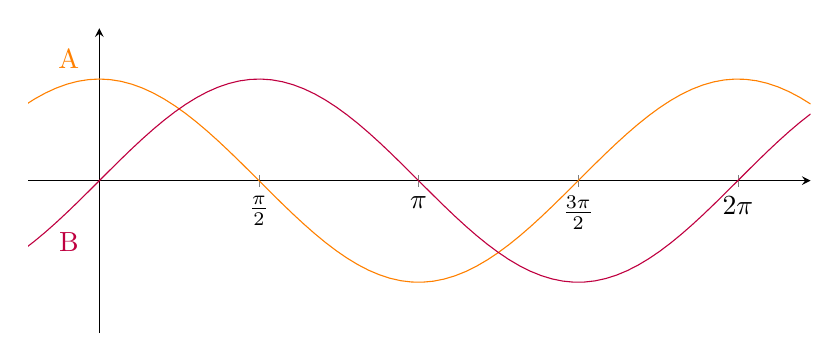
\begin{tikzpicture}
	\begin{axis}[
		axis lines=middle,
		unit vector ratio*=1 1,
		scale=1.45,
		ymin=-1.5, ymax=1.5, xmin=-0.7, xmax=7,
		domain=-3.5:7,
		samples=100,
		ymajorticks=false,
		xtick={ 0.5*pi, pi, 1.5*pi, 2*pi},
		xticklabels={$\frac{\pi}{2}$, $\pi$, $\frac{3\pi}{2}$, $2\pi$},
		disabledatascaling
	]
	\addplot [mark=none, orange] {sin(deg(x+0.5*pi))};
	\node[orange] at (-0.3,1.2) {A};
	
	\addplot [mark=none, purple] {sin(deg(x))};
	\node[purple] at (-0.3,-0.6) {B};
\end{axis}
\end{tikzpicture}\end{center}

\noindent
Przyjrzyjmy się możliwej konstrukcji silnika zasilanego dwufazowo z dwoma biegunami (złożonego z mogącego obracać się magnesu trwałego i dwóch cewek podłączonych po jednej do każdej z faz – cewki tworzą elektromagnesy przyciągające bądź odpychające obracający się magnes trwały):

\begin{center} \begin{tabular}{c|c|c|c|c|c|c|c}
	$t=0$ & &
	$t=\frac{\pi}{2}$ & &
	$t=\pi$ & &
	$t=\frac{3\pi}{2}$ &\\
	\twoPhase{blue}{gray}{90}  & \twoPhase{blue!30}{blue!30}{45} &
	\twoPhase{gray}{blue}{0}   & \twoPhase{red!30}{blue!30}{-45} &
	\twoPhase{red}{gray}{-90}  & \twoPhase{red!30}{red!30}{-135} &
	\twoPhase{gray}{red}{-180} & \twoPhase{blue!30}{red!30}{-225}
\end{tabular} \end{center}

Warto tutaj zauważyć że tak zbudowany silnik jest dość niesymetryczny i dodatkowo może mieć problemy ze startem z pewnych pozycji.
Dlatego w praktyce w takim silniku zastosowano by 4 bieguny (cewki) poprzez dodanie biegunów A' i B' mających działanie odwrotne do A i B (co jest łatwo uzyskać nawijając cewkę „w drugą stronę”):

\begin{center} \begin{tabular}{c|c|c|c|c|c|c|c}
	$t=0$ & &
	$t=\frac{\pi}{2}$ & &
	$t=\pi$ & &
	$t=\frac{3\pi}{2}$ &\\
	\fourPhase{blue}{gray}{red}{gray}{90}  & \fourPhase{blue!30}{blue!30}{red!30}{red!30}{45} &
	\fourPhase{gray}{blue}{gray}{red}{0}   & \fourPhase{red!30}{blue!30}{blue!30}{red!30}{-45} &
	\fourPhase{red}{gray}{blue}{gray}{-90}  & \fourPhase{red!30}{red!30}{blue!30}{blue!30}{-135} &
	\fourPhase{gray}{red}{gray}{blue}{-180} & \fourPhase{blue!30}{red!30}{red!30}{blue!30}{-225}
\end{tabular} \end{center}

Warto jednak zauważyć iż uzyskaliśmy w ten sposób układ 4 fazowy:

\begin{center} 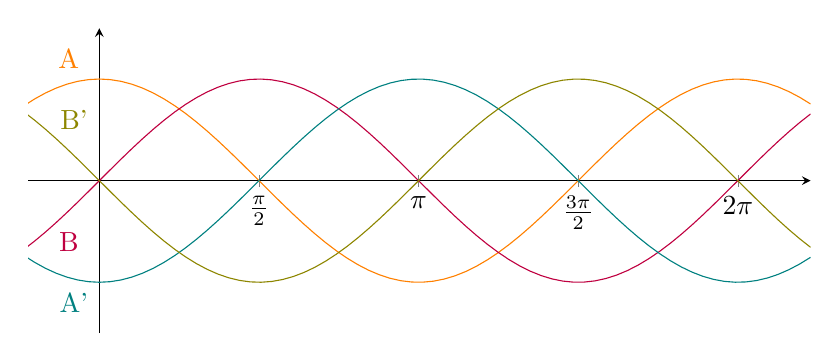
\begin{tikzpicture}
	\begin{axis}[
		axis lines=middle,
		unit vector ratio*=1 1,
		scale=1.45,
		ymin=-1.5, ymax=1.5, xmin=-0.7, xmax=7,
		domain=-3.5:7,
		samples=100,
		ymajorticks=false,
		xtick={ 0.5*pi, pi, 1.5*pi, 2*pi},
		xticklabels={$\frac{\pi}{2}$, $\pi$, $\frac{3\pi}{2}$, $2\pi$},
		disabledatascaling
	]
	\addplot [mark=none, orange] {sin(deg(x+0.5*pi))};
	\node[orange] at (-0.3,1.2) {A};
	
	\addplot [mark=none, purple] {sin(deg(x))};
	\node[purple] at (-0.3,-0.6) {B};
	
	\addplot [mark=none, teal] {sin(deg(x+1.5*pi))};
	\node[teal] at (-0.25,-1.2) {A'};
	
	\addplot [mark=none, olive] {sin(deg(x+pi))};
	\node[olive] at (-0.25,0.6) {B'};
\end{axis}
\end{tikzpicture}\end{center}

Układ dwufazowy był historycznie stosowany z okablowaniem 4 żyłowym (ze względu na brak równoważenia prądu w przewodzie neutralnym).
Został jednak całkowicie wyparty przez układ trójfazowy.

\subsection{podzielona faza}

Układ \href{https://en.wikipedia.org/wiki/Split-phase_electric_power}{podzielonej fazy} można uzyskać stosując transformator z pojedynczym uzwojeniem pierwotnym i podzielonym uzwojeniem wtórnym:

\begin{center} \begin{adjustbox}{scale=0.75} \begin{tikzpicture}
	\begin{scope}[xshift=-1cm]\begin{axis}[
		scale=0.7,
		ymin=-1.5, ymax=1.5, xmin=0, xmax=2*pi,
		domain=0:2*pi,
		samples=100,
		ymajorticks=false,
		xmajorticks=false,
		axis line style={draw=none},
	]
		\addplot [mark=none] {sin(deg(x))};
	\end{axis}\end{scope}

	\begin{scope}[xshift=4cm]
		% primary
		\draw(0, 0)  to [short, o-] +(1, 0)
			to [inductor, bipoles/americaninductor/width=2, bipoles/americaninductor/coils=10]  +(0, 3.5)
			to [short, -o] +(-1, 0);

		% core
		\draw[thick] (1.33, 0.5) -- (1.33, 3);
		\draw[thick] (1.53, 0.5) -- (1.53, 3);

		%secondary
		\draw(3, 0)  to [short, o-] +(-1, 0)
			to [inductor]  +(0, 1.75)
			to [inductor]  +(0, 1.75)
			to [short, -o] +(1, 0);
		\draw(2,1.75) to [short, *-] +(1, 0);
	\end{scope}

	\begin{scope}[xshift=7cm, yshift=.35cm]\begin{axis}[
		scale=0.5,
		ymin=-3, ymax=3, xmin=0, xmax=2*pi,
		domain=0:2*pi,
		samples=100,
		ymajorticks=false,
		xmajorticks=false,
		axis line style={draw=none},
	]
		\addplot [orange, mark=none] {-1.5+sin(deg(x+pi))};
		\addplot [purple, mark=none] { 1.5+sin(deg(x))};
	\end{axis}\end{scope}
\end{tikzpicture} \end{adjustbox} \end{center}

\begin{center} 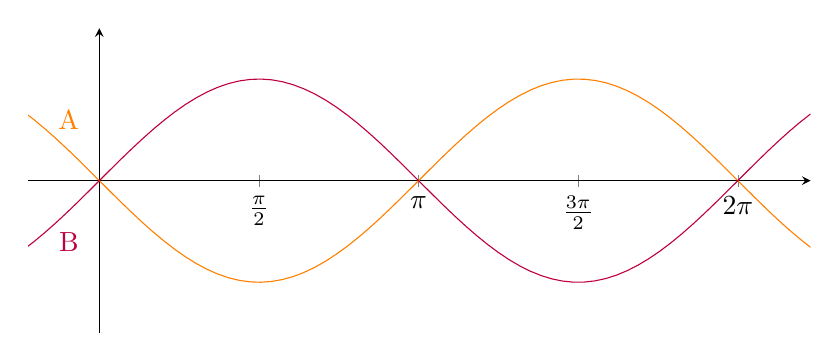
\begin{tikzpicture}
	\begin{axis}[
		axis lines=middle,
		unit vector ratio*=1 1,
		scale=1.45,
		ymin=-1.5, ymax=1.5, xmin=-0.7, xmax=7,
		domain=-3.5:7,
		samples=100,
		ymajorticks=false,
		xtick={ 0.5*pi, pi, 1.5*pi, 2*pi},
		xticklabels={$\frac{\pi}{2}$, $\pi$, $\frac{3\pi}{2}$, $2\pi$},
		disabledatascaling
	]
	\addplot [mark=none, orange] {sin(deg(x+pi))};
	\node[orange] at (-0.3,0.6) {A};
	
	\addplot [mark=none, purple] {sin(deg(x))};
	\node[purple] at (-0.3,-0.6) {B};
\end{axis}
\end{tikzpicture}\end{center}

\noindent
W układzie takim nie jest możliwe użycie silnika wielofazowego:
\begin{center} \begin{tabular}{c|c|c|c|c|c|c|c}
	$t=0$ &
	$t=\frac{\pi}{2}$ &
	$t=\pi$ &
	$t=\frac{3\pi}{2}$\\
	\twoPhase{gray}{gray}{0} &
	\twoPhase{blue}{red}{90} &
	\twoPhase{gray}{gray}{90} &
	\twoPhase{red}{blue}{0}
\end{tabular} \end{center}

\noindent
Uzyskaliśmy co najwyżej oscylacje pomiędzy pozycją $t=\frac{\pi}{2}$ i $t=\frac{3\pi}{2}$.
Jeżeli zastosowalibyśmy cewki w „przeciw fazie” to też nie uzyskamy poprawy:

\begin{center} \begin{tabular}{c|c|c|c|c|c|c|c}
	$t=0$ &
	$t=\frac{\pi}{2}$ &
	$t=\pi$ &
	$t=\frac{3\pi}{2}$\\
	\fourPhase{gray}{gray}{gray}{gray}{-45} &
	\fourPhase{blue}{red}{red}{blue}{135} &
	\fourPhase{gray}{gray}{gray}{gray}{135} &
	\fourPhase{red}{blue}{blue}{red}{-45}
\end{tabular} \end{center}

\noindent
Dzieje się tak dlatego że A' = B oraz B' = A, czyli nie uzyskaliśmy niczego nowego tym zabiegiem.
Wynika to z faktu iż zasada działania tych dodatkowych biegunów silnika jest analogiczna do podzielonej fazy\footnote{
	Można powiedzieć że poprzednio stosując zabieg z użyciem odwrotnie nawiniętych cewek uzyskaliśmy podział faz A i B na połowy, co dało nam układ 4 fazowy.
}, ale podzielonej fazy nie możemy już bardziej podzielić – w wyniku podziału dostaniemy takie same przesunięcia co w wyniku pierwszego podziału.

Podzielona faza może zostać uzyskana także w układzie trójfazowym typu \href{https://en.wikipedia.org/wiki/High-leg_delta}{\textit{High-leg delta}}:

\begin{center} \begin{adjustbox}{scale=1.2} \begin{tikzpicture}
\draw (0,0) to (0,-1.7) node[ground]{};
\draw (0,0) to [inductor, align=left, l=\hspace{-5pt}\color{blue}\scriptsize$U_{AN}\eq$120~V]  (-2.0, 0)
      to [inductor, bipoles/americaninductor/width=1.6, bipoles/americaninductor/coils=8, l=\color{red}\scriptsize$U_{AC}\eq240$~V] (0, 3.0)
      to [inductor, bipoles/americaninductor/width=1.6, bipoles/americaninductor/coils=8, l=\color{red}\scriptsize$U_{BC}\eq240$~V] (2.0, 0)
      to [inductor, align=left, l=\color{blue}\scriptsize$U_{BN}\eq$120~V] (0, 0);
\draw(0,-1.3) to [short, *-o] +(1, 0) node[anchor=west]{N};
\draw(-2.0,0) to [short, *-o] +(-1,0) node[anchor=east]{A};
\draw(2.0, 0) to [short, *-o] +(1, 0) node[anchor=west]{B};
\draw(0, 3)   to [short, *-o] +(0, .7) node[anchor=south]{C};

\draw[red,<->] (-1.8,0.2) -- node[yshift=6pt] {\scriptsize$U_{AB}\eq$240~V} (1.8,0.2);
\draw[orange,<->] (0,0.05) -- node[rotate=90, yshift=6pt] {\scriptsize$U_{CN}\eq$208~V} (0, 2.9);
\end{tikzpicture} \end{adjustbox} \end{center}

Warto zauważyć, iż w układzie podzielonej fazy napięcie międzyfazowe jest zwykłą sumą napięć fazowych. W pokazanym przykładzie: $$U_{AB_{sk}} = 240{\rm ~V} = U_{AN_{sk}} + U_{BN_{sk}} = 120{\rm ~V} + 120{\rm ~V}$$

Układ ten jest powszechnie stosowany w Ameryce Północnej.
Trochę więcej na jego temat (oraz na temat instalacji elektrycznych w USA) można dowiedzieć się z: \url{https://www.youtube.com/watch?v=fJeRabV5hNU}.

\subsection{trzy fazy}

Najpowszechniej stosowanym system wytwarzania i dystrybucji energii elektrycznej jest \href{https://en.wikipedia.org/wiki/Three-phase_electric_power}{układ trójfazowy}, w którym przesunięcie pomiędzy kolejnymi fazami wynosi $\frac{2\pi}{3}$.

\newcommand{\threesixPhase}[7] {
	\begin{adjustbox}{scale=0.43}
	\begin{tikzpicture}
		\tikzstyle{fullrotate}=[rotate=##1,nodes={rotate=##1}]
		\tikzstyle{coil}=[align=center, minimum height=0.7cm, minimum width=0.7cm, fill=##1]
		
		\node[coil=#1] at (0,1.7) {A};
		\begin{scope}[fullrotate=-120]
			\node[coil=#2] at (0,1.7) {B};
		\end{scope}
		\begin{scope}[fullrotate=120]
			\node[coil=#3] at (0,1.7) {C};
		\end{scope}
		
		\begin{scope}[fullrotate=180]
			\node[coil=#4] at (0,1.7) {\aprim};
		\end{scope}
		\begin{scope}[fullrotate=60]
			\node[coil=#5] at (0,1.7) {\bprim};
		\end{scope}
		\begin{scope}[fullrotate=-60]
			\node[coil=#6] at (0,1.7) {\cprim};
		\end{scope}
		
		\node[coil=none] at (0,1.9) {};
		
		\begin{scope}[fullrotate=#7]
			\fill[blue] (-1,-0.35) rectangle (0,0.35);
			\node at (-0.5,0) {N};
			\fill[red] (0,-0.35) rectangle (1,0.35);
			\node at (0.5,0) {S};
		\end{scope}
	\end{tikzpicture}
	\end{adjustbox}
}
\newcommand{\threePhase}[4] {
	\def\aprim{}\def\bprim{}\def\cprim{}
	\threesixPhase{#1}{#2}{#3}{none}{none}{none}{#4}
}
\newcommand{\sixPhase}[7] {
	\def\aprim{A'}\def\bprim{B'}\def\cprim{C'}
	\threesixPhase{#1}{#2}{#3}{#4}{#5}{#6}{#7}
}


\begin{center} 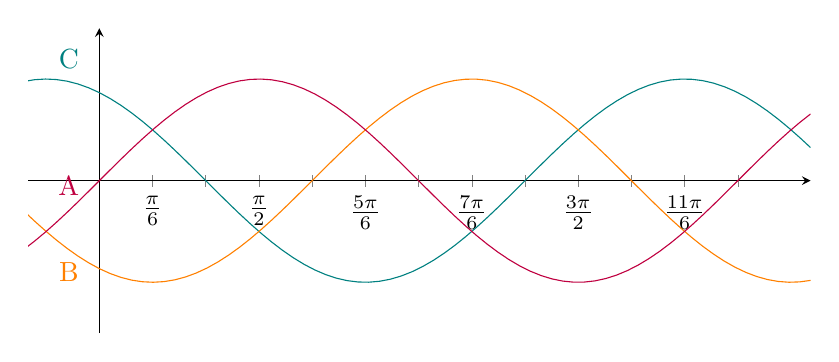
\begin{tikzpicture}
	\begin{axis}[
		axis lines=middle,
		unit vector ratio*=1 1,
		scale=1.45,
		ymin=-1.5, ymax=1.5, xmin=-0.7, xmax=7,
		domain=-3.5:7,
		samples=100,
		ymajorticks=false,
		xtick={pi/6, 2*pi/6, 3*pi/6, 4*pi/6, 5*pi/6, 6*pi/6, 7*pi/6, 8*pi/6, 9*pi/6, 10*pi/6, 11*pi/6, 12*pi/6},
		xticklabels={$\frac{\pi}{6}$, ~, $\frac{\pi}{2}$, ~, $\frac{5\pi}{6}$, ~, $\frac{7\pi}{6}$, ~, $\frac{3\pi}{2}$, ~, $\frac{11\pi}{6}$, ~},
		disabledatascaling
	]
	\addplot [mark=none, teal] {sin(deg(x+2*pi/3))};
	\node[teal] at (-0.3,1.2) {C};
	
	\addplot [mark=none, orange] {sin(deg(x+4*pi/3))};
	\node[orange] at (-0.3,-0.9) {B};
	
	\addplot [mark=none, purple] {sin(deg(x))};
	\node[purple] at (-0.3,-0.05) {A};
\end{axis}
\end{tikzpicture}\end{center}

\noindent
Przyjrzyjmy się możliwej konstrukcji silnika zasilanego trójfazowo:

\begin{center} \begin{tabular}{c|c|c|c|c|c}
	$t=\frac{\pi}{6}$ &
	$t=\frac{\pi}{2}$ &
	$t=\frac{5\pi}{6}$ &
	$t=\frac{7\pi}{6}$ &
	$t=\frac{3\pi}{2}$ &
	$t=\frac{11\pi}{6}$\\
	\threePhase{blue!25}{red}{blue!25}{150} &
	\threePhase{blue}{red!25}{red!25}{90} &
	\threePhase{blue!25}{blue!25}{red}{30} &
	\threePhase{red!25}{blue}{red!25}{-30} &
	\threePhase{red}{blue!25}{blue!25}{-90} &
	\threePhase{red!25}{red!25}{blue}{-150}
\end{tabular} \end{center}
%
Oczywiście tutaj także możemy wprowadzić dodatkowe bieguny A', B' i C' o działaniu przeciwny do A, B i C (poprzez odwrotne nawinięcie ich cewek):
%
\begin{center} \begin{tabular}{c|c|c|c|c|c}
	$t=\frac{\pi}{6}$ &
	$t=\frac{\pi}{2}$ &
	$t=\frac{5\pi}{6}$ &
	$t=\frac{7\pi}{6}$ &
	$t=\frac{3\pi}{2}$ &
	$t=\frac{11\pi}{6}$\\
	\sixPhase{blue!25}{red}{blue!25}{red!25}{blue}{red!25}{150} &
	\sixPhase{blue}{red!25}{red!25}{red}{blue!25}{blue!25}{90} &
	\sixPhase{blue!25}{blue!25}{red}{red!25}{red!25}{blue}{30} &
	\sixPhase{red!25}{blue}{red!25}{blue!25}{red}{blue!25}{-30} &
	\sixPhase{red}{blue!25}{blue!25}{blue}{red!25}{red!25}{-90} &
	\sixPhase{red!25}{red!25}{blue}{blue!25}{blue!25}{red}{-150}
\end{tabular} \end{center}
%
Co daje nam funkcjonalny odpowiednik układu 6cio fazowego o przesunięciu $\frac{\pi}{3}$:
%
\begin{center} 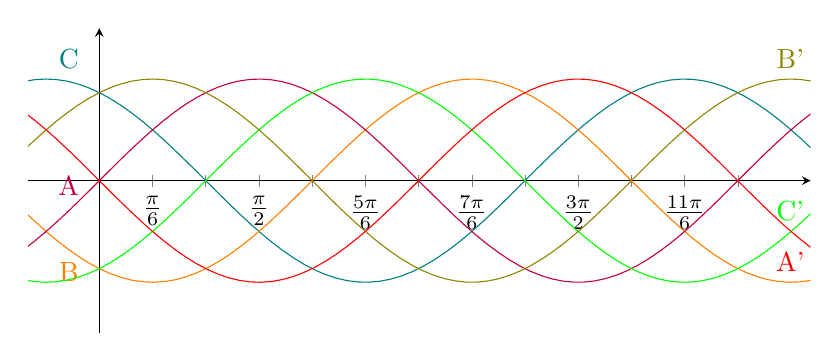
\begin{tikzpicture}
	\begin{axis}[
		axis lines=middle,
		unit vector ratio*=1 1,
		scale=1.45,
		ymin=-1.5, ymax=1.5, xmin=-0.7, xmax=7,
		domain=-3.5:7,
		samples=100,
		ymajorticks=false,
		xtick={pi/6, 2*pi/6, 3*pi/6, 4*pi/6, 5*pi/6, 6*pi/6, 7*pi/6, 8*pi/6, 9*pi/6, 10*pi/6, 11*pi/6, 12*pi/6},
		xticklabels={$\frac{\pi}{6}$, ~, $\frac{\pi}{2}$, ~, $\frac{5\pi}{6}$, ~, $\frac{7\pi}{6}$, ~, $\frac{3\pi}{2}$, ~, $\frac{11\pi}{6}$, ~},
		disabledatascaling
	]
	\addplot [mark=none, teal] {sin(deg(x+2*pi/3))};
	\node[teal] at (-0.3,1.2) {C};
	
	\addplot [mark=none, orange] {sin(deg(x+4*pi/3))};
	\node[orange] at (-0.3,-0.9) {B};
	
	\addplot [mark=none, purple] {sin(deg(x))};
	\node[purple] at (-0.3,-0.05) {A};
	
	
	\addplot [mark=none, green] {sin(deg(x+5*pi/3))};
	\node[green] at (6.8, -0.3) {C'};
	
	\addplot [mark=none, olive] {sin(deg(x+7*pi/3))};
	\node[olive] at (6.8,1.2) {B'};
	
	\addplot [mark=none, red] {sin(deg(x+pi))};
	\node[red] at (6.8,-0.8) {A'};
	
\end{axis}
\end{tikzpicture}\end{center}
%
Warto jednak zauważyć że 3 fazy są najmniejszą liczbą faz, dla których taki zabieg nie jest konieczny.


\subsubsection{napięcie międzyfazowe}

\noindent
Pamiętając że napięcie to różnica potencjałów\footnote{i że napięcie fazowe w postaci sinusoidy, jest różnicą potencjału przewodu fazowego i przewodu neutralnego}, możemy obliczyć napięcie między fazowe:
	$$U_{AN} = V_A - V_N \qquad U_{BN} = V_B - V_N \qquad U_{AB} = V_A - V_B$$
	$$U_{AB} = (U_{AN} + V_N) - (U_{BN} + V_N) = U_{AN} - U_{BN}$$
Jak widzimy jest ono różnicą napięć fazowych (a nie ich sumą).
Należy jednak mieć na uwadze że jest to różnica przesuniętych w fazie sinusoid (a nie stałych wartości i z tego powodu napięcie to nie wynosi zero):
	$$U_{AB} = U_{AN} - U_{BN} = U_0 \cdot \sin(t) - U_0 \cdot \sin\left( t + \frac{2\pi}{3} \right)$$
	$$U_{AB} = U_0 \left( \sin(t) - \sin\left( t + \frac{2\pi}{3} \right) \right)$$
gdzie $U_0$ to amplituda napięcia fazowego.
%
Korzystając z tożsamości trygonometrycznej: $\sin(x) - \sin(y) = 2 \cdot \sin(\frac{x - y}{2}) \cdot \cos(\frac{x + y}{2})$ otrzymujemy:
	$$U_{AB} = U_0 \cdot 2 \cdot \sin\left( \frac{t - (t + \frac{2\pi}{3})}{2} \right) \cdot \cos\left( \frac{t + (t + \frac{2\pi}{3})}{2} \right)$$
	$$U_{AB} = U_0 \cdot 2 \cdot \sin\left( -\frac{\pi}{3} \right) \cdot \cos\left( t + \frac{\pi}{3} \right) = U_0 \cdot 2 \cdot \frac{\sqrt{3}}{2} \cdot \cos\left( t + \frac{\pi}{3} \right)$$
	$$U_{AB} = \sqrt{3} \cdot U_0 \cdot \cos\left( t + \frac{\pi}{3} \right)$$
Obliczenia dla pozostałych napięć międzyfazowych są analogiczne.
Widzimy zatem że napięcie międzyfazowe będzie przesunięte względem napięć rozważanych faz i będzie miało amplitudę (a zatem także wartość międzyszczytową i skuteczną) $\sqrt{3}$ raza większą od wartości napięcia fazowego.

\begin{center} \begin{adjustbox}{scale=0.75} \begin{tikzpicture}
	\begin{axis}[
		axis lines=middle,
		unit vector ratio*=1 1,
		scale=2.5,
		ymin=-2.2, ymax=2.2, xmin=-3.2, xmax=7,
		domain=-3.5:7,
		samples=100,
		ytick={ -sqrt(3), -1, 1, sqrt(3)},
		yticklabels={$-\sqrt{3} \cdot U_0$, $-U_0$, $U_0$, $\sqrt{3} \cdot U_0$},
		xtick={ 0.5*pi, pi, 1.5*pi, 2*pi},
		xticklabels={$\frac{\pi}{2}$, $\pi$, $\frac{3\pi}{2}$, $2\pi$},
		disabledatascaling
	]
	\addplot [mark=none, orange] {sin(deg(x+2*pi/3))};
	\node[orange] at (-1.9,0.45) {A};
	
	\addplot [mark=none, purple] {sin(deg(x))};
	\node[purple] at (-1.9,-0.75) {B};
	
	\addplot [mark=none, blue] {sin(deg(x+2*pi/3)) - sin(deg(x))};
	\node[blue] at (-2.02,1.4) {A-B};
	
	%\addplot [mark=none, red] {sqrt(3) * cos(deg(x+pi/3))};
	%\node[red] at (-2.02,1.4) {A-B};
\end{axis}
\end{tikzpicture} \end{adjustbox} \end{center}


\subsubsection{trójkąt-gwiazda}

Istnieją i są stosowane dwa sposoby połączeń uzwojeń (zarówno silników, generatorów, jak i transformatorów) w systemach trójfazowych - trójkąt (delta $\Delta$) i gwiazda (star, Y).
Przy połączeniu w trójkąt nie dostajemy (przy generatorze, uzwojeniu wtórnym transformatora) / nie używamy (przy silnikach) przewodu neutralnego – operujemy tylko na napięciach międzyfazowych.
W przypadku połączenia w gwiazdę możemy (ale nie musimy) korzystać z punktu neutralnego.

Typowo transformatory energetyczne z średniego na niskie napięcie działają w układzie trójkąt-gwiazda, czyli po stronie pierwotnej (średniego napięcia) uzwojenia łączone są w trójką, a po stronie wtórnej (400V) w gwiazdę.
Dzięki temu dostępny jest po stronie wtórnej punkt neutralny i możliwe jest korzystanie zarówno z napięć międzyfazowych (400V) jak i jednofazowych L-N (230V).

\begin{center} \begin{adjustbox}{scale=1.0} \begin{tikzpicture}

	\begin{scope}[xshift=-4cm,yshift=-1.7cm]
		\ctikzset{bipoles/americaninductor/width=1.6, bipoles/americaninductor/coils=8}
		\draw (-2.0,0) to [inductor] (2.0, 0) to [inductor] (0, 3.0) to [inductor] (-2.0,0);
		\draw(-2.0,0) to [short, *-o] +(-1,0) node[anchor=east]{A};
		\draw(2.0, 0) to [short, *-o] +(1, 0) node[anchor=west]{B};
		\draw(0, 3)   to [short, *-o] +(0, .7) node[anchor=south]{C};
		
		\draw[red,<->] (-2.0,-0.2) -- node[below] {\scriptsize$U_{AB}\eq$400~V} (2.0,-0.2);
		\draw[red,<->] (-2.15,0.15) -- node[above, sloped] {\scriptsize$U_{AC}\eq$400~V} (-0.22,3);
		\draw[red,<->] (2.15,0.15) -- node[above, sloped] {\scriptsize$U_{BC}\eq$400~V} (0.22,3);
		
		\node at (0,-1.3) {\bf trójkąt (delta, $\Delta$)};
	\end{scope}

	\begin{scope}[xshift=4cm]
		\draw (0,0) to [inductor] (-1.3, -1.3) to [short, -o] +(-0.9,0) node[anchor=east]{A};
		\draw (1.3, -1.3) to [inductor] (0,0); \draw (1.3, -1.3) to [short, -o] +(0.9, 0) node[anchor=west]{B};
		\draw (0,0) to [inductor] (0, 1.8) to [short, -o] +(0, 0.3) node[anchor=south]{C};
		\draw(0,0) to [short, *-o] +(0, -2.0) node[anchor=north]{N};
		
		\draw[red,<->] (-2.3,-1.7) -- node[above] {\scriptsize$U_{AB}\eq$400~V} (2.3,-1.7);
		\draw[red,<->] (-2.25,-1.05) -- node[above, sloped] {\scriptsize$U_{AC}\eq$400~V} (-0.22,2.1);
		\draw[red,<->] (2.25,-1.05) -- node[above, sloped] {\scriptsize$U_{BC}\eq$400~V} (0.22,2.1);
		
		\draw[blue,<->] (-1.35,-1.05) -- node[above, sloped] {\scriptsize$U_{AN}\eq$230~V} (-0.35, -0.05);
		\draw[blue,<->] (1.35,-1.05) -- node[above, sloped] {\scriptsize$U_{BN}\eq$230~V} (0.35, -0.05);
		\draw[blue,<->] (0.15,0.05) -- node[below, sloped, align=left, font=\scriptsize] {~$U_{CN}\eq$\\~230~V} (0.15, 1.7);
		
		\node at (0,-3) {\bf gwiazda (star, Y)};
	\end{scope}
\end{tikzpicture} \end{adjustbox} \end{center}
%
Należy zauważyć że podłączenie uzwojeń (o takiej samej impedancji) w gwiazdę skutkuje mniejszym poborem prądu niż podłączenie ich w trójkąt.
Jest to efektem tego że w połączeniu typu gwiazda napięcia na poszczególnych uzwojeniach są mniejsze ($\sqrt{3}$ raza) niż w przypadku połączenia w trójkąt (230V vs 400V).
